\documentclass[12pt]{report}

%% Good fonts for PDF
\usepackage[cyr]{aeguill}

%% Package for page headers
\usepackage{fancyhdr}

%% Package to include graphics
%% Comment for DVI
\usepackage[pdftex]{graphicx}

%% Index
\usepackage{makeidx}
\makeindex

%% Figures formats: jpeg or pdf
%% Comment for DVI
\DeclareGraphicsExtensions{.jpg,.pdf}

%% Package to create Hyperdocuments
%% Comment for DVI
\usepackage[pdftex,colorlinks=true,linkcolor=blue,citecolor=blue,urlcolor=blue]{hyperref}

%% Package to control printed area size
\usepackage{anysize}
%% ...by defining margins {left}{right}{top}{bottom}
\marginsize{22mm}{14mm}{12mm}{25mm}

%% Package used to include a bibliography
\usepackage{natbib}

%% R for real numbers
\usepackage{amssymb}

%% User defined commands

%% Figure reference
\newcommand{\figref}[1]{figure~\ref{#1}}

%% Equation reference
\newcommand{\Ref}[1]{(\ref{#1})}

%% Emphasize a word or a group of words
\newcommand{\empha}[1]{\textit{\textbf{#1}}}

%% Derivation operators
\newcommand{\D}{\partial}
\newcommand{\Dt}{\partial_t}
\newcommand{\Dx}{\partial_x}
\newcommand{\Dy}{\partial_y}

\newcommand{\bv}{\mathbf{v}}
\newcommand{\bx}{\mathbf{x}}
\newcommand{\bl}{\mathbf{l}}
\newcommand{\br}{\mathbf{r}}
\newcommand{\bg}{\mathbf{g}}

\usepackage{url}

% Scilab macros
\newcommand{\scifunction}[1]{\textit{#1}}

% To highlight source code
\usepackage{listings}

\lstdefinelanguage{scilabscript}%
  {morekeywords={abcd,abinv,abort,abs,acoshm,acosh,acosm,acos,addcolor,%
      addf,addinter,addmenu,add_edge,add_node,adj2sp,adj_lists,aff2ab,%
      amell,analpf,analyze,ans,apropos,arc_graph,arc_number,argn,arhnk,%
      arl2,arma2p,armac,armax1,armax,arma,arsimul,artest,articul,ascii,%
      asinhm,asinh,asinm,asin,atanhm,atanh,atanm,atan,augment,auread,%
      auwrite,balanc,balreal,bandwr,basename,bdiag,besseli,besselj,%
      besselk,bessely,best_match,bezout,bifish,bilin,binomial,black,%
      bloc2exp,bloc2ss,bode,bool2s,boolean,boucle,break,bstap,buttmag,%
      bvode,cainv,calerf,calfrq,call,canon,casc,case,ccontrg,cdfbet,%
      cdfbin,cdfchi,cdfchn,cdffnc,cdff,cdfgam,cdfnbn,cdfnor,cdfpoi,%
      cdft,ceil,center,cepstrum,chaintest,chain_struct,champ1,champ,%
      chart,chdir,cheb1mag,cheb2mag,check_graph,check_io,chepol,chfact,%
      chol,chsolve,circuit,classmarkov,clean,clearfun,clearglobal,%
      clear,close,cls2dls,cmb_lin,cmndred,cmoment,code2str,coeff,coffg,%
      coff,colcompr,colcomp,colinout,colormap,colregul,companion,comp,%
      cond,conj,connex,contour2di,contour2d,contourf,contour,%
      contract_edge,contrss,contr,cont_frm,cont_mat,convex_hull,convol,%
      convstr,con_nodes,copfac,copy,correl,corr,coshm,cosh,cosm,cos,%
      cotg,cothm,coth,covar,csim,cspect,ctr_gram,cumprod,cumsum,%
      curblock,cycle_basis,czt,c_link,dasrt,dassl,datafit,date,dbphi,%
      dcf,ddp,debug,dec2hex,deff,definedfields,degree,delbpt,%
      delete_arcs,delete_nodes,delete,delip,delmenu,demos,denom,%
      derivative,derivat,des2ss,des2tf,determ,detr,det,dft,dhinf,%
      dhnorm,diag,diary,diff,diophant,dirname,dispbpt,dispfiles,disp,%
      dlgamma,double,dragrect,drawaxis,drawlater,drawnow,draw,driver,%
      dscr,dsearch,dsimul,dtsi,dt_ility,duplicate,edge_number,%
      edit_curv,edit_graph_menus,edit_graph,edit,eigenmarkov,ell1mag,%
      elseif,else,emptystr,endfunction,end,eqfir,eqiir,equil1,equil,%
      ereduc,erfcx,erfc,erf,errbar,errcatch,errclear,error,eval3dp,%
      eval3d,eval,evans,evstr,excel2sci,execstr,exec,exists,exit,expm,%
      exp,external,eye,fac3d,factors,faurre,fchamp,fcontour2d,fcontour,%
      fec,feedback,feval,ffilt,fftshift,fft,fgrayplot,figure,fileinfo,%
      file,filter,findm,findobj,findx0BD,find_freq,find_path,find,%
      findABCD,findAC,findBD,findBDK,findR,fit_dat,fix,floor,flts,foo,%
      formatman,format,fort,for,fourplan,fplot2d,fplot3d1,fplot3d,%
      fprintf,fprintfMat,frep2tf,freq,freson,frexp,frfit,frmag,fscanf,%
      fscanfMat,fsfirlin,fsolve,fspecg,fstabst,fstair,ftest,ftuneq,%
      fullrfk,fullrf,full,fun2string,funcprot,functions,function,%
      funptr,fusee,gainplot,gamitg,gammaln,gamma,gcare,gcd,gcf,%
      genfac3d,genlib,genmarkov,gen_net,geom3d,geomean,getblocklabel,%
      getcolor,getcurblock,getcwd,getdate,getd,getenv,getfield,getfont,%
      getf,getio,getlinestyle,getmark,getpid,getscicosvars,getsymbol,%
      getvalue,getversion,get_function_path,get,gfare,gfrancis,girth,%
      givens,glever,glist,global,glue,gpeche,graduate,grand,%
      graphics_entities,graph_2_mat,graph_center,graph_complement,%
      graph_diameter,graph_power,graph_simp,graph_sum,graph_union,%
      graph-list,graycolormap,grayplot,graypolarplot,grep,group,%
      gr_menu,gschur,gsort,gspec,gstacksize,gtild,g_margin,h2norm,halt,%
      hamilton,hankelsv,hank,harmean,havewindow,help,hermit,hess,%
      hex2dec,hilb,hinf,hist3d,histplot,horner,host,hotcolormap,%
      householder,hrmt,htrianr,hypermat,h_cl,h_inf_st,h_inf,h_norm,%
      iconvert,icon_edit,ieee,if,iirgroup,iirlp,iir,ilib_build,%
      ilib_compile,ilib_for_link,ilib_gen_gateway,ilib_gen_loader,%
      ilib_gen_Make,imag,impl,imrep2ss,imult,im_inv,inistate,input,%
      int16,int2d,int32,int3d,int8,intc,intdec,integrate,interpln,%
      interp,intersci,intersect,intg,intl,intppty,intsplin,inttrap,%
      inttype,int,invr,invsyslin,inv_coeff,inv,iqr,isdef,isdir,isequal,%
      iserror,isglobal,isinf,isnan,isoview,isreal,is_connex,jmat,%
      justify,kalm,karmarkar,kernel,keyboard,knapsack,kpure,krac2,%
      kroneck,kron,lasterror,lattn,lattp,lcf,lcmdiag,lcm,ldivf,ldiv,%
      leastsq,legends,length,leqr,levin,lev,lex_sort,lft,lgfft,library,%
      lib,lin2mu,lincos,lindquist,lines,line_graph,linfn,linf,link,%
      linmeq,linpro,linsolve,linspace,lin,listfiles,list,lmisolver,%
      lmitool,loadmatfile,loadplots,loadwave,load_graph,load,locate,%
      log10,log1p,log2,logm,logspace,log,lotest,lqe,lqg2stan,lqg_ltr,%
      lqg,lqr,lsq,lsslist,lstcat,lstsize,ltitr,ludel,lufact,luget,%
      lusolve,lu,lyap,macglov,macr2lst,macrovar,macro,mad,make_graph,%
      make_index,manedit,man,mapsound,markp2ss,matfile2sci,matrix,%
      mat_2_graph,maxi,max_cap_path,max_clique,max_flow,max,mclearerr,%
      mclose,meanf,mean,median,meof,mese,mesh2d,mfft,mfile2sci,mgeti,%
      mgetl,mgetstr,mget,milk_drop,mine,mini,minreal,minss,%
      min_lcost_cflow,min_lcost_flow1,min_lcost_flow2,min_qcost_flow,%
      min_weight_tree,min,mlist,mode,modulo,moment,mopen,move,%
      mps2linpro,mputl,mputstr,mput,mrfit,msd,mseek,mtell,mtlb_load,%
      mtlb_mode,mtlb_save,mtlb_sparse,mu2lin,mulf,mvvacov,m_circle,%
      names,nand2mean,nanmax,nanmeanf,nanmean,nanmedian,nanmin,%
      nanstdev,nansum,narsimul,ndims,nearfloat,nehari,neighbors,%
      netclose,netwindows,netwindow,newest,newfun,nextpow2,nf3d,nfreq,%
      nlev,nnz,nodes_2_path,nodes_degrees,node_number,noisegen,norm,%
      null,numdiff,numer,nyquist,obscont1,obscont,observer,obsvss,%
      obsv_mat,obs_gram,odedc,odedi,odeoptions,ode_discrete,ode_root,%
      ode,oldload,oldsave,ones,optim,orth,param3d1,param3d,%
      paramfplot2d,parrot,part,pathconvert,path_2_nodes,pause,pbig,%
      pdiv,pen2ea,pencan,penlaur,perctl,perfect_match,pertrans,pfss,%
      phasemag,phc,pinv,pipe_network,playsnd,plot2d1,plot2d2,plot2d3,%
      plot2d4,plot2d,plot3d1,plot3d2,plot3d3,plot3d,plotframe,%
      plotprofile,plot_graph,plot,plzr,pmodulo,pol2des,pol2str,pol2tex,%
      polarplot,polar,polfact,poly,portr3d,portrait,power,ppol,prbs_a,%
      predecessors,predef,printf,printing,print,prod,profile,projsl,%
      projspec,proj,psmall,pspect,pvm_addhosts,pvm_barrier,pvm_bcast,%
      pvm_bufinfo,pvm_config,pvm_delhosts,pvm_error,pvm_exit,%
      pvm_f772sci,pvm_getinst,pvm_gettid,pvm_get_timer,pvm_gsize,%
      pvm_halt,pvm_joingroup,pvm_kill,pvm_lvgroup,pvm_mytid,pvm_parent,%
      pvm_probe,pvm_recv,pvm_reduce,pvm_sci2f77,pvm_send,pvm_set_timer,%
      pvm_spawn_independent,pvm_spawn,pvm_start,pvm_tasks,%
      pvm_tidtohost,pvm,pwd,p_margin,qassign,qr,quapro,quart,quaskro,%
      quit,randpencil,rand,range,rankqr,rank,rat,rcond,rdivf,read4b,%
      readb,readc_,readmps,read,real,recur,reglin,regress,remezb,remez,%
      repfreq,replot,residu,resume,return,riccati,riccsl,ricc,ric_desc,%
      rlist,roots,rotate,round,routh_t,rowcompr,rowcomp,rowinout,%
      rowregul,rowshuff,rpem,rref,rtitr,rubberbox,salesman,savewave,%
      save_graph,save,scaling,scanf,schur,sci2exp,sci2for,sci2map,%
      sciargs,scicosim,scicos,scifunc_block,sd2sci,secto3d,select,%
      semidef,sensi,setbpt,seteventhandler,setfield,setmenu,%
      setscicosvars,set,sfact,sgrid,shortest_path,showprofile,%
      show_arcs,show_graph,show_nodes,sident,signm,sign,simp_mode,simp,%
      sincd,sinc,sinc,sinhm,sinh,sinm,sin,size,sm2des,sm2ss,smooth,%
      solve,sorder,sort,sound,sp2adj,spaninter,spanplus,spantwo,sparse,%
      spchol,spcompack,specfact,spec,speye,spget,splin,split_edge,%
      spones,sprand,sprintf,spzeros,sqroot,sqrtm,sqrt,squarewave,%
      square,srfaur,srkf,ss2des,ss2ss,ss2tf,sscanf,sskf,ssprint,ssrand,%
      stabil,stacksize,standard_define,standard_draw,standard_input,%
      standard_origin,standard_output,startup,stdevf,stdev,steadycos,%
      str2code,strange,strcat,strindex,strings,string,stripblanks,%
      strong_connex,strong_con_nodes,strsubst,st_deviation,st_ility,%
      subf,subgraph,subplot,successors,sum,supernode,sva,svd,svplot,%
      sylm,sylv,sysconv,sysdiag,sysfact,syslin,syssize,systems,system,%
      systmat,tabul,tangent,tanhm,tanh,tanm,tan,tdinit,testmatrix,%
      texprint,tf2des,tf2ss,then,thrownan,timer,time_id,titlepage,%
      tk_getdir,tk_getfile,tlist,toeplitz,tokenpos,tokens,trace,%
      translatepaths,trans_closure,trans,trfmod,trianfml,tril,trimmean,%
      trisolve,triu,trzeros,typename,typeof,type,uicontrol,uimenu,%
      uint16,uint32,uint8,ui_observer,ulink,unglue,union,unique,unix_g,%
      unix_s,unix_w,unix_x,unix,unobs,unsetmenu,user,varargin,%
      varargout,variancef,variance,varn,warning,wavread,wavwrite,%
      wcenter,wfir,what,whereami,whereis,where,while,whos,who_user,who,%
      wiener,wigner,window,winsid,with_gtk,with_pvm,with_texmacs,%
      with_tk,writb,write4b,write,xarcs,xarc,xarrows,xaxis,xbasc,%
      xbasimp,xbasr,xchange,xclear,xclea,xclick,xclip,xdel,xend,xfarcs,%
      xfarc,xfpolys,xfpoly,xfrect,xgetech,xgetfile,xgetmouse,xget,%
      xgraduate,xgrid,xinfo,xinit,xlfont,xload,xname,xnumb,xpause,%
      xpolys,xpoly,xrects,xrect,xrpoly,xs2fig,xs2gif,xs2ppm,xs2ps,%
      xsave,xsegs,select,xsetech,xsetm,xset,xstringb,xstringl,xstring,%
      xtape,xtitle,x_choices,x_choose,x_dialog,x_matrix,x_mdialog,%
      x_message_modeless,x_message,yulewalk,zeropen,zeros,zgrid,zpbutt,%
      zpch1,zpch2,zpell,mfprintf,mfscanf,mprintf,mscanf,msprintf,%
      msscanf,mucomp,%
      ABSBLK_f,AFFICH_f,ANDLOG_f,ANIMXY_f,BIGSOM_f,CLINDUMMY_f,CLKIN_f,%
      CLKINV_f,CLKOUT_f,CLKOUTV_f,CLKSOM_f,CLKSOMV_f,CLKSPLIT_f,%
      CLOCK_f,CLR_f,CLSS_f,CONST_f,COSBLK_f,CURV_f,DELAY_f,DELAYV_f,%
      DEMUX_f,DLR_f,DLRADAPT_f,DLSS_f,EVENTSCOPE_f,EVTDLY_f,EVTGEN_f,%
      EXPBLK_f,G_make,GAIN_f,GAINBLK_f,GENERAL_f,GENERIC_f,GENSIN_f,%
      GENSQR_f,HALT_f,IFTHEL_f,IN_f,INTEGRAL_f,INTRP2BLK_f,INTRPLBLK_f,%
      INVBLK_f,LOGBLK_f,LOOKUP_f,Matplot1,Matplot,MAX_f,MCLOCK_f,%
      MFCLCK_f,MIN_f,MUX_f,NDcost,NEGTOPOS_f,OUT_f,POSTONEG_f,POWBLK_f,%
      PROD_f,QUANT_f,RAND_f,READC_f,REGISTER_f,RELAY_f,RFILE_f,%
      ScilabEval,Sfgrayplot,Sgrayplot,SAMPLEHOLD_f,SAT_f,SAWTOOTH_f,%
      SCOPE_f,SCOPXY_f,SELECT_f,SINBLK_f,SOM_f,SPLIT_f,STOP_f,SUPER_f,%
      TANBLK_f,TCLSS_f,TEXT_f,TIME_f,TK_EvalFile,TK_EvalStr,TK_GetVar,%
      TK_SetVar,TRASH_f,WFILE_f,WRITEC_f,ZCROSS_f,%
      \%asn,\%helps,\%k,\%sn},%
   alsoletter=\%,% chmod
   sensitive,%
   morecomment=[l]//,%
   morestring=[b]",%
   morestring=[m]'%
   numbers=none,%
   basicstyle=\tiny,%
   keywordstyle=\bfseries,%
   commentstyle=\bfseries,%
   showspaces=false,%
   stringstyle=\bfseries
  }[keywords,comments,strings]%

\lstdefinelanguage{matlabscript}%
  {morekeywords={gt,lt,gt,lt,amp,abs,acos,acosh,acot,acoth,acsc,acsch,%
      all,angle,ans,any,asec,asech,asin,asinh,atan,atan2,atanh,auread,%
      auwrite,axes,axis,balance,bar,bessel,besselk,bessely,beta,%
      betainc,betaln,blanks,bone,break,brighten,capture,cart2pol,%
      cart2sph,caxis,cd,cdf2rdf,cedit,ceil,chol,cla,clabel,clc,clear,%
      clf,clock,close,colmmd,Colon,colorbar,colormap,ColorSpec,colperm,%
      comet,comet3,compan,compass,computer,cond,condest,conj,contour,%
      contour3,contourc,contrast,conv,conv2,cool,copper,corrcoef,cos,%
      cosh,cot,coth,cov,cplxpair,cputime,cross,csc,csch,csvread,%
      csvwrite,cumprod,cumsum,cylinder,date,dbclear,dbcont,dbdown,%
      dbquit,dbstack,dbstatus,dbstep,dbstop,dbtype,dbup,ddeadv,ddeexec,%
      ddeinit,ddepoke,ddereq,ddeterm,ddeunadv,deblank,dec2hex,deconv,%
      del2,delete,demo,det,diag,diary,diff,diffuse,dir,disp,dlmread,%
      dlmwrite,dmperm,dot,drawnow,echo,eig,ellipj,ellipke,else,elseif,%
      end,engClose,engEvalString,engGetFull,engGetMatrix,engOpen,%
      engOutputBuffer,engPutFull,engPutMatrix,engSetEvalCallback,%
      engSetEvalTimeout,engWinInit,eps,erf,erfc,erfcx,erfinv,error,%
      errorbar,etime,etree,eval,exist,exp,expint,expm,expo,eye,fclose,%
      feather,feof,ferror,feval,fft,fft2,fftshift,fgetl,fgets,figure,%
      fill,fill3,filter,filter2,find,findstr,finite,fix,flag,fliplr,%
      flipud,floor,flops,fmin,fmins,fopen,for,format,fplot,fprintf,%
      fread,frewind,fscanf,fseek,ftell,full,function,funm,fwrite,fzero,%
      gallery,gamma,gammainc,gammaln,gca,gcd,gcf,gco,get,getenv,%
      getframe,ginput,global,gplot,gradient,gray,graymon,grid,griddata,%
      gtext,hadamard,hankel,help,hess,hex2dec,hex2num,hidden,hilb,hist,%
      hold,home,hostid,hot,hsv,hsv2rgb,if,ifft,ifft2,imag,image,%
      imagesc,Inf,info,input,int2str,interp1,interp2,interpft,inv,%
      invhilb,isempty,isglobal,ishold,isieee,isinf,isletter,isnan,%
      isreal,isspace,issparse,isstr,jet,keyboard,kron,lasterr,lcm,%
      legend,legendre,length,lin2mu,line,linspace,load,log,log10,log2,%
      loglog,logm,logspace,lookfor,lower,ls,lscov,lu,magic,matClose,%
      matDeleteMatrix,matGetDir,matGetFp,matGetFull,matGetMatrix,%
      matGetNextMatrix,matGetString,matlabrc,matlabroot,matOpen,%
      matPutFull,matPutMatrix,matPutString,max,mean,median,menu,mesh,%
      meshc,meshgrid,meshz,mexAtExit,mexCallMATLAB,mexdebug,%
      mexErrMsgTxt,mexEvalString,mexFunction,mexGetFull,mexGetMatrix,%
      mexGetMatrixPtr,mexPrintf,mexPutFull,mexPutMatrix,mexSetTrapFlag,%
      min,more,movie,moviein,mu2lin,mxCalloc,mxCopyCharacterToPtr,%
      mxCopyComplex16ToPtr,mxCopyInteger4ToPtr,mxCopyPtrToCharacter,%
      mxCopyPtrToComplex16,mxCopyPtrToInteger4,mxCopyPtrToReal8,%
      mxCopyReal8ToPtr,mxCreateFull,mxCreateSparse,mxCreateString,%
      mxFree,mxFreeMatrix,mxGetIr,mxGetJc,mxGetM,mxGetN,mxGetName,%
      mxGetNzmax,mxGetPi,mxGetPr,mxGetScalar,mxGetString,mxIsComplex,%
      mxIsFull,mxIsNumeric,mxIsSparse,mxIsString,mxIsTypeDouble,%
      mxSetIr,mxSetJc,mxSetM,mxSetN,mxSetName,mxSetNzmax,mxSetPi,%
      mxSetPr,NaN,nargchk,nargin,nargout,newplot,nextpow2,nnls,nnz,%
      nonzeros,norm,normest,null,num2str,nzmax,ode23,ode45,orient,orth,%
      pack,pascal,patch,path,pause,pcolor,pi,pink,pinv,plot,plot3,%
      pol2cart,polar,poly,polyder,polyeig,polyfit,polyval,polyvalm,%
      pow2,print,printopt,prism,prod,pwd,qr,qrdelete,qrinsert,quad,%
      quad8,quit,quiver,qz,rand,randn,randperm,rank,rat,rats,rbbox,%
      rcond,real,realmax,realmin,refresh,rem,reset,reshape,residue,%
      return,rgb2hsv,rgbplot,rootobject,roots,rose,rosser,rot90,rotate,%
      round,rref,rrefmovie,rsf2csf,save,saxis,schur,sec,sech,semilogx,%
      semilogy,set,setstr,shading,sign,sin,sinh,size,slice,sort,sound,%
      spalloc,sparse,spaugment,spconvert,spdiags,specular,speye,spfun,%
      sph2cart,sphere,spinmap,spline,spones,spparms,sprandn,sprandsym,%
      sprank,sprintf,spy,sqrt,sqrtm,sscanf,stairs,startup,std,stem,%
      str2mat,str2num,strcmp,strings,strrep,strtok,subplot,subscribe,%
      subspace,sum,surf,surface,surfc,surfl,surfnorm,svd,symbfact,%
      symmmd,symrcm,tan,tanh,tempdir,tempname,terminal,text,tic,title,%
      toc,toeplitz,trace,trapz,tril,triu,type,uicontrol,uigetfile,%
      uimenu,uiputfile,unix,unwrap,upper,vander,ver,version,view,%
      viewmtx,waitforbuttonpress,waterfall,wavread,wavwrite,what,%
      whatsnew,which,while,white,whitebg,who,whos,wilkinson,wk1read,%
      wk1write,xlabel,xor,ylabel,zeros,zlabel,zoom},%
   sensitive,%
   morecomment=[l]\%,%
   basicstyle=\tiny,%
   morestring=[m]'%
  }[keywords,comments,strings]%

\usepackage{algorithmic}

% To allow one bibliograph by chapter
%\usepackage[sectionbib]{chapterbib}
\usepackage{url}

% Maths shortcuts 
\newcommand{\RR}{\mathbb{R}}
\newcommand{\CC}{\mathbb{C}}

% For symbol degree
\DeclareTextSymbol{\degre}{T1}{6}





\begin{document}
%% User defined page headers
\pagestyle{fancyplain}
\renewcommand{\chaptermark}[1]{\markboth{\chaptername\ \thechapter. #1}{}}
\renewcommand{\sectionmark}[1]{\markright{\thesection. #1}}
\lhead[]{\fancyplain{}{\bfseries\leftmark}}
\rhead[]{\fancyplain{}{\bfseries\thepage}}
\cfoot{}

%% User defined figure legends
\makeatletter
\def\figurename{{\protect\sc \protect\small\bfseries Fig.}}
\def\f@ffrench{\protect\figurename\space{\protect\small\bf \thefigure}\space}
\let\fnum@figure\f@ffrench%
\let\captionORI\caption
\def\caption#1{\captionORI{\rm\small #1}}
\makeatother

%% First page
\thispagestyle{empty}
{
\begin{center}
%% Comment for DVI

\includegraphics[height=40mm]{scilab_logo}
\vskip2cm

%% Empty space between the box and the text
\fboxsep6mm
%% Box thickness
\fboxrule1.3pt
\Huge
$$\fbox{$
  \begin{array}{c}
  \textbf{Nelder-Mead}\\
  \textbf{User's Manual}\\
  \textbf{-- The Fminsearch Function --}\\
  \end{array}
  $}
$$
\end{center}

\vskip1cm

\begin{center}
\begin{large}
Micha\"el BAUDIN
\end{large}
\end{center}

\vskip2cm


\vskip1cm


\begin{flushright}
Version 0.3 \\
September 2009
\end{flushright}



\clearpage


\tableofcontents

\chapter{The \scifunction{fminsearch} function}
\index{fminsearch}

In this chapter, we analyze the implementation of the \scifunction{fminsearch}
which is provided in Scilab. In the first part, we describe the specific 
choices of this implementation with respect to the Nelder-Mead algorithm.
In the second part, we present some numerical experiments which 
allows to check that the feature is behaving as expected, by comparison 
to Matlab's \scifunction{fminsearch}.

\section{\scifunction{fminsearch}'s algorithm}

In this section, we analyse the specific choices used in 
\scifunction{fminsearch}'s algorithm. We detail what specific variant
of the Nelder-Mead algorithm is performed, what initial simplex is used,
the default number of iterations and the termination criteria.

\subsection{The algorithm}

The algorithm used is the Nelder-Mead algorithm. This corresponds to the 
"variable" value of the "-method" option of the \scifunction{neldermead}.
The "non greedy" version is used, that is, the expansion point is 
accepted only if it improves over the reflection point.

\subsection{The initial simplex}
\index{Pfeffer, L.}
\index{Fan, Ellen}

The fminsearch algorithm uses a special initial simplex, which is an 
heuristic depending on the initial guess. The strategy chosen by 
fminsearch corresponds to the -simplex0method flag of the neldermead 
component, with the "pfeffer" method. It is associated with the -
simplex0deltausual = 0.05 and -simplex0deltazero = 0.0075 parameters. 
Pfeffer's method is an heuristic which is presented in "Global 
Optimization Of Lennard-Jones Atomic Clusters" by Ellen Fan \cite{Fan2002}. 
It is due to L. Pfeffer at Stanford. See in the help of optimsimplex for more 
details.

\subsection{The number of iterations}

In this section, we present the default values for the number of 
iterations in fminsearch.

The options input argument is an optionnal data structure which can 
contain the options.MaxIter field. It stores the maximum number of 
iterations. The default value is 200n, where n is the number of 
variables. The factor 200 has not been chosen by chance, but is the 
result of experiments performed against quadratic functions with 
increasing space dimension.

This result is presented in "Effect of dimensionality on the nelder-mead 
simplex method" by Lixing Han and Michael Neumann \cite{HanNeumann2006}. This paper is based 
on Lixing Han's PhD, "Algorithms in Unconstrained Optimization" \cite{Han2000}. The 
study is based on numerical experiment with a quadratic function where 
the number of terms depends on the dimension of the space (i.e. the 
number of variables). Their study shows that the number of iterations 
required to reach the tolerance criteria is roughly 100n. Most 
iterations are based on inside contractions. Since each step of the 
Nelder-Mead algorithm only require one or two function evaluations, the 
number of required function evaluations in this experiment is also 
roughly 100n.

\subsection{The termination criteria}

The algorithm used by \scifunction{fminsearch} uses a particular 
termination criteria, based both on the absolute size of the 
simplex and the difference of the function values in the simplex.
This termination criteria corresponds to the "-tolssizedeltafvmethod"
termination criteria of the \scifunction{neldermead} component.

The size of the simplex is computed with the $\sigma-+$ method,
which corresponds to the "sigmaplus" method of the \scifunction{optimsimplex}
component. The tolerance associated with this criteria is 
given by the "TolX" parameter of the \scifunction{options} data structure.
Its default value is 1.e-4.

The function value difference is the difference 
between the highest and the lowest function value in the simplex.
The tolerance associated with this criteria is given by the 
"TolFun" parameter of the \scifunction{options} data structure.
Its default value is 1.e-4.

\section{Numerical experiments}

In this section, we analyse the behaviour of Scilab's \scifunction{fminsearch}
function, by comparison of Matlab's \scifunction{fminsearch}. We especially analyse 
the results of the optimization, so that we can check that the algorithm
is indeed behaving the same way, even if the implementation is completely 
different. 

We consider the unconstrained optimization problem \cite{citeulike:1903787}
\begin{eqnarray}
\min f(\bx)
\end{eqnarray}
where $\bx\in\RR^2$ and the objective function $f$ is defined by 
\begin{eqnarray}
f(\bx) = 100*(x_2-x_1^2)^2+(1-x_1)^2.
\end{eqnarray}
The initial guess is 
\begin{eqnarray}
\bx^0 = ( -1.2 , 1.)^T,
\end{eqnarray}
where the function value is 
\begin{eqnarray}
f(\bx^0) = 24.2.
\end{eqnarray}
The global solution of this problem is
\begin{eqnarray}
\bx^\star = ( 1 , 1.)^T
\end{eqnarray}
where the function value is 
\begin{eqnarray}
f(\bx^\star) = 0.
\end{eqnarray}

\subsection{Algorithm and numerical precision}

In this section, we are concerned by the comparison of the behavior 
of the two algorithms. We are going to check that the algorithms 
produces the same intermediate and final results.
We also analyze the numerical precision of the results,
by detailing the number of significant digits.

To make a more living presentation of this topic, we will 
include small scripts which allow to produce the output 
that we are going to analyze. Because of the similarity of the languages, 
in order to avoid confusion, we will specify, for each script, the language 
we use by a small comment. Scripts and outputs written in Matlab's language will begin with 
\lstset{language=matlabscript}
\begin{lstlisting}
% Matlab
% ...
\end{lstlisting}
while script written in Scilab's language will begin with
\lstset{language=scilabscript}
\begin{lstlisting}
// Scilab
// ...
\end{lstlisting}

The following Matlab script allows to see the behaviour of Matlab's \scifunction{fminsearch}
function on Rosenbrock's test case.

\lstset{language=matlabscript}
\begin{lstlisting}
% Matlab
format long
banana = @(x)100*(x(2)-x(1)^2)^2+(1-x(1))^2;
[x,fval,exitflag,output] = fminsearch(banana,[-1.2, 1])
output.message
\end{lstlisting}

When this script is launched in Matlab, the following output is 
produced.

\lstset{language=matlabscript}
\begin{lstlisting}
>> % Matlab
>> format long
>> banana = @(x)100*(x(2)-x(1)^2)^2+(1-x(1))^2;
>> [x,fval] = fminsearch(banana,[-1.2, 1])
>> [x,fval,exitflag,output] = fminsearch(banana,[-1.2, 1])
x =
   1.000022021783570   1.000042219751772
fval =
     8.177661197416674e-10
exitflag =
     1
output =
    iterations: 85
     funcCount: 159
     algorithm: 'Nelder-Mead simplex direct search'
       message: [1x194 char]
>> output.message
ans =
Optimization terminated:
the current x satisfies the termination criteria using
OPTIONS.TolX of 1.000000e-04
and F(X) satisfies the convergence criteria using
OPTIONS.TolFun of 1.000000e-04
\end{lstlisting}

The following Scilab script allows to solve the problem with Scilab's 
\scifunction{fminsearch}.

\lstset{language=scilabscript}
\begin{lstlisting}
// Scilab
format(25)
function y = banana (x)
  y = 100*(x(2)-x(1)^2)^2 + (1-x(1))^2;
endfunction
[x , fval , exitflag , output] = fminsearch ( banana , [-1.2 1] )
output.message
\end{lstlisting}

The output associated with this Scilab script is the following.

\lstset{language=scilabscript}
\begin{lstlisting}
-->// Scilab
-->format(25)
-->function y = banana (x)
-->  y = 100*(x(2)-x(1)^2)^2 + (1-x(1))^2;
-->endfunction
-->[x , fval , exitflag , output] = fminsearch ( banana , [-1.2 1] )
 output  =
   algorithm: "Nelder-Mead simplex direct search"
   funcCount: 159
   iterations: 85
   message: [3x1 string]
 exitflag  =
    1.  
 fval  =
    0.0000000008177661099387  
 x  =
    1.0000220217835567027009    1.0000422197517710998227  
-->output.message
 ans  =
 
!Optimization terminated:                                                              !
!                                                                                      !
!the current x satisfies the termination criteria using OPTIONS.TolX of 1.000000e-004  !
!                                                                                      !
!and F(X) satisfies the convergence criteria using OPTIONS.TolFun of 1.000000e-004     !
\end{lstlisting}

Because the two softwares do not use the same formatting rules 
to produce their outputs, we must perform additionnal checking 
in order to check our results.

The following Scilab script displays the results with 16 significant digits.

\lstset{language=scilabscript}
\begin{lstlisting}
// Scilab
// Print the result with 15 significant digits
mprintf ( "%.15e" , fval );
mprintf ( "%.15e %.15e" , x(1) , x(2) );
\end{lstlisting}

The previous script produces the following output.

\lstset{language=scilabscript}
\begin{lstlisting}
-->// Scilab
-->mprintf ( "%.15e" , fval );
8.177661099387146e-010 
-->mprintf ( "%.15e %.15e" , x(1) , x(2) );
1.000022021783557e+000 1.000042219751771e+000 
\end{lstlisting}

These results are reproduced verbatim in the table 
\ref{fig-fminsearch-comparison}.

\begin{figure}[htbp]
\begin{center}
\begin{tabular}{|l|l|l|}
\hline
Matlab Iterations & 85 &\\
Scilab Iterations & 85 &\\
\hline
Matlab Function Evaluations & 159 &\\
Scilab Function Evaluations & 159 &\\
\hline
Matlab $\bx^\star$ & 1.000022021783570   & 1.000042219751772 \\
Scilab $\bx^\star$ & 1.000022021783557e+000 & 1.000042219751771e+000 \\
\hline
Matlab $f(\bx^\star)$ & 8.177661197416674e-10 &\\
Scilab $f(\bx^\star)$ & 8.177661099387146e-010  &\\
\hline
\end{tabular}
\end{center}
\caption{Numerical experiment with Rosenbrock's function -- Comparison of 
results produced by Matlab and Scilab.}
\label{fig-fminsearch-comparison}
\end{figure}

We must compute the common number of significant digits 
in order to check the consistency of the results.
The following Scilab script computes the relative error 
between Scilab and Matlab results.

\lstset{language=scilabscript}
\begin{lstlisting}
// Scilab
// Compare the result
xmb = [1.000022021783570   1.000042219751772 ];
err = norm(x - xmb) / norm(xmb);
mprintf ( "Relative Error on x : %e\n", err );
fmb = 8.177661197416674e-10;
err = abs(fval - fmb) / abs(fmb);
mprintf ( "Relative Error on f : %e\n", err );
\end{lstlisting}

The previous script produces the following output.

\lstset{language=scilabscript}
\begin{lstlisting}
// Scilab
Relative Error on x : 9.441163e-015
Relative Error on f : 1.198748e-008
\end{lstlisting}

We must take into account for the floating point implementations 
of both Matlab and Scilab. In both these numerical softwares,
double precision floating point numbers are used, i.e. the relative 
precision is both these softwares is $\epsilon \approx 10^{-16}$. 
That implies that there are approximately 16 significant digits.
Therefore, the relative error on $x$, which is equivalent to 15
significant digits, is acceptable. 

Therefore, the result is as close as possible to the result produced 
by Matlab. More specifically :
\begin{itemize}
\item the optimum $x$ is the same up to 15 significant digits,
\item the function value at optimum is the same up to 8 significant digits,
\item the number of iterations is the same,
\item the number of function evaluations is the same,
\item the exit flag is the same,
\item the content of the output is the same (but the string is not 
display the same way).
\end{itemize}

The output of the two functions is the same. 
We must now check that the algorithms performs the same way,
that is, produces the same intermediate steps.

The following Matlab script allows to get deeper information by printing a message at each iteration
with the "Display" option.

\index{optimset}

\lstset{language=matlabscript}
\begin{lstlisting}
% Matlab
opt = optimset('Display','iter');
[x,fval,exitflag,output] = fminsearch(banana,[-1.2, 1] , opt );
\end{lstlisting}

The previous script produces the following output.

\lstset{language=matlabscript}
\begin{lstlisting}
% Matlab
 Iteration   Func-count     min f(x)         Procedure
     0            1             24.2         
     1            3            20.05         initial simplex
     2            5           5.1618         expand
     3            7           4.4978         reflect
     4            9           4.4978         contract outside
     5           11          4.38136         contract inside
     6           13          4.24527         contract inside
     7           15          4.21762         reflect
     8           17          4.21129         contract inside
     9           19          4.13556         expand
    10           21          4.13556         contract inside
    11           23          4.01273         expand
    12           25          3.93738         expand
    13           27          3.60261         expand
    14           28          3.60261         reflect
    15           30          3.46622         reflect
    16           32          3.21605         expand
    17           34          3.16491         reflect
    18           36          2.70687         expand
    19           37          2.70687         reflect
    20           39          2.00218         expand
    21           41          2.00218         contract inside
    22           43          2.00218         contract inside
    23           45          1.81543         expand
    24           47          1.73481         contract outside
    25           49          1.31697         expand
    26           50          1.31697         reflect
    27           51          1.31697         reflect
    28           53           1.1595         reflect
    29           55          1.07674         contract inside
    30           57         0.883492         reflect
    31           59         0.883492         contract inside
    32           61         0.669165         expand
    33           63         0.669165         contract inside
    34           64         0.669165         reflect
    35           66         0.536729         reflect
    36           68         0.536729         contract inside
    37           70         0.423294         expand
    38           72         0.423294         contract outside
    39           74         0.398527         reflect
    40           76          0.31447         expand
    41           77          0.31447         reflect
    42           79         0.190317         expand
    43           81         0.190317         contract inside
    44           82         0.190317         reflect
    45           84          0.13696         reflect
    46           86          0.13696         contract outside
    47           88         0.113128         contract outside
    48           90          0.11053         contract inside
    49           92          0.10234         reflect
    50           94         0.101184         contract inside
    51           96        0.0794969         expand
    52           97        0.0794969         reflect
    53           98        0.0794969         reflect
    54          100        0.0569294         expand
    55          102        0.0569294         contract inside
    56          104        0.0344855         expand
    57          106        0.0179534         expand
    58          108        0.0169469         contract outside
    59          110       0.00401463         reflect
    60          112       0.00401463         contract inside
    61          113       0.00401463         reflect
    62          115      0.000369954         reflect
    63          117      0.000369954         contract inside
    64          118      0.000369954         reflect
    65          120      0.000369954         contract inside
    66          122     5.90111e-005         contract outside
    67          124     3.36682e-005         contract inside
    68          126     3.36682e-005         contract outside
    69          128     1.89159e-005         contract outside
    70          130     8.46083e-006         contract inside
    71          132     2.88255e-006         contract inside
    72          133     2.88255e-006         reflect
    73          135     7.48997e-007         contract inside
    74          137     7.48997e-007         contract inside
    75          139     6.20365e-007         contract inside
    76          141     2.16919e-007         contract outside
    77          143     1.00244e-007         contract inside
    78          145     5.23487e-008         contract inside
    79          147     5.03503e-008         contract inside
    80          149      2.0043e-008         contract inside
    81          151     1.12293e-009         contract inside
    82          153     1.12293e-009         contract outside
    83          155     1.12293e-009         contract inside
    84          157     1.10755e-009         contract outside
    85          159     8.17766e-010         contract inside
 
Optimization terminated:
 the current x satisfies the termination criteria using OPTIONS.TolX of 1.000000e-004 
 and F(X) satisfies the convergence criteria using OPTIONS.TolFun of 1.000000e-004 
\end{lstlisting}

The following Scilab script set the "Display" option to "iter" and 
run the \scifunction{fminsearch} function.
\index{optimset}

\lstset{language=scilabscript}
\begin{lstlisting}
// Scilab
opt = optimset ( "Display" , "iter" );
[x , fval , exitflag , output] = fminsearch ( banana , [-1.2 1] , opt );
\end{lstlisting}

\lstset{language=scilabscript}
\begin{lstlisting}
// Scilab
 Iteration   Func-count     min f(x)         Procedure
     0            3             24.2            
     1            3            20.05         initial simplex     
     2            5         5.161796         expand              
     3            7         4.497796         reflect             
     4            9         4.497796         contract outside    
     5           11        4.3813601         contract inside     
     6           13        4.2452728         contract inside     
     7           15        4.2176247         reflect             
     8           17        4.2112906         contract inside     
     9           19        4.1355598         expand              
    10           21        4.1355598         contract inside     
    11           23        4.0127268         expand              
    12           25        3.9373812         expand              
    13           27         3.602606         expand              
    14           28         3.602606         reflect             
    15           30        3.4662211         reflect             
    16           32        3.2160547         expand              
    17           34        3.1649126         reflect             
    18           36        2.7068692         expand              
    19           37        2.7068692         reflect             
    20           39        2.0021824         expand              
    21           41        2.0021824         contract inside     
    22           43        2.0021824         contract inside     
    23           45        1.8154337         expand              
    24           47        1.7348144         contract outside    
    25           49        1.3169723         expand              
    26           50        1.3169723         reflect             
    27           51        1.3169723         reflect             
    28           53        1.1595038         reflect             
    29           55        1.0767387         contract inside     
    30           57        0.8834921         reflect             
    31           59        0.8834921         contract inside     
    32           61        0.6691654         expand              
    33           63        0.6691654         contract inside     
    34           64        0.6691654         reflect             
    35           66        0.5367289         reflect             
    36           68        0.5367289         contract inside     
    37           70        0.4232940         expand              
    38           72        0.4232940         contract outside    
    39           74        0.3985272         reflect             
    40           76        0.3144704         expand              
    41           77        0.3144704         reflect             
    42           79        0.1903167         expand              
    43           81        0.1903167         contract inside     
    44           82        0.1903167         reflect             
    45           84        0.1369602         reflect             
    46           86        0.1369602         contract outside    
    47           88        0.1131281         contract outside    
    48           90        0.1105304         contract inside     
    49           92        0.1023402         reflect             
    50           94        0.1011837         contract inside     
    51           96        0.0794969         expand              
    52           97        0.0794969         reflect             
    53           98        0.0794969         reflect             
    54          100        0.0569294         expand              
    55          102        0.0569294         contract inside     
    56          104        0.0344855         expand              
    57          106        0.0179534         expand              
    58          108        0.0169469         contract outside    
    59          110        0.0040146         reflect             
    60          112        0.0040146         contract inside     
    61          113        0.0040146         reflect             
    62          115        0.0003700         reflect             
    63          117        0.0003700         contract inside     
    64          118        0.0003700         reflect             
    65          120        0.0003700         contract inside     
    66          122        0.0000590         contract outside    
    67          124        0.0000337         contract inside     
    68          126        0.0000337         contract outside    
    69          128        0.0000189         contract outside    
    70          130        0.0000085         contract inside     
    71          132        0.0000029         contract inside     
    72          133        0.0000029         reflect             
    73          135        0.0000007         contract inside     
    74          137        0.0000007         contract inside     
    75          139        0.0000006         contract inside     
    76          141        0.0000002         contract outside    
    77          143        0.0000001         contract inside     
    78          145        5.235D-08         contract inside     
    79          147        5.035D-08         contract inside     
    80          149        2.004D-08         contract inside     
    81          151        1.123D-09         contract inside     
    82          153        1.123D-09         contract outside    
    83          155        1.123D-09         contract inside     
    84          157        1.108D-09         contract outside    
    85          159        8.178D-10         contract inside     

Optimization terminated:
 the current x satisfies the termination criteria using OPTIONS.TolX of 1.000000e-004
 and F(X) satisfies the convergence criteria using OPTIONS.TolFun of 1.000000e-004
\end{lstlisting}

We check that the two softwares produces indeed the same intermediate results in terms
of iteration, function evaluations, function values and type of steps.
The only difference is the iteration \#0, which is associated with 
function evaluation \#1 in Matlab and with function evaluation \#3 in Scilab.
This is because Scilab calls back the output function once the initial
simplex is computed, which requires 3 function evaluations. 

\subsection{Output and plot functions}

In this section, we check that the output and plot features of the 
\scifunction{fminsearch} function are the same.
We also check that the fields and the content of the \scivar{optimValues}
data structure and the \scivar{state} variable are the same in 
both languages.

The following output function plots in the current graphic 
window the value of the current parameter $\bx$.
It also unloads the content of the \scivar{optimValues}
data structure and prints a message in the console.
To let Matlab load that script, save the content in a 
.m file, in a directory known by Matlab.

\lstset{language=matlabscript}
\begin{lstlisting}
% Matlab
function stop = outfun(x, optimValues, state)
stop = false;
hold on;
plot(x(1),x(2),'.');
fc = optimValues.funccount;
fv = optimValues.fval;
it = optimValues.iteration;
pr = optimValues.procedure;
disp(sprintf ( '%d %e %d -%s- %s\n' , fc , fv , it , pr , state ))
drawnow
\end{lstlisting}

The following Matlab script allows to perform the optimization
so that the output function is called back at each iteration.
\index{optimset}

\lstset{language=matlabscript}
\begin{lstlisting}
% Matlab
options = optimset('OutputFcn', @outfun);
[x fval] = fminsearch(banana, [-1.2, 1], options)
\end{lstlisting}

This produces the plot which is presented in figure \ref{fig-fminsearch-matlab-outputfun}.

\begin{figure}
\begin{center}
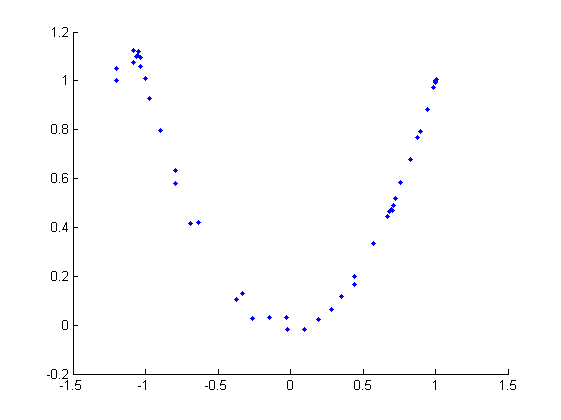
\includegraphics[width=10cm]{fminsearch/testFminsearchPlotMatlab.png}
\end{center}
\caption{Plot produced by Matlab's fminsearch, with customized output function.}
\label{fig-fminsearch-matlab-outputfun}
\end{figure}

Matlab also prints the following messages in the console.

\lstset{language=matlabscript}
\begin{lstlisting}
% Matlab
1 2.420000e+001 0 -- init
1 2.420000e+001 0 -- iter
3 2.005000e+001 1 -initial simplex- iter
5 5.161796e+000 2 -expand- iter
7 4.497796e+000 3 -reflect- iter
9 4.497796e+000 4 -contract outside- iter
11 4.381360e+000 5 -contract inside- iter
13 4.245273e+000 6 -contract inside- iter
[...]
149 2.004302e-008 80 -contract inside- iter
151 1.122930e-009 81 -contract inside- iter
153 1.122930e-009 82 -contract outside- iter
155 1.122930e-009 83 -contract inside- iter
157 1.107549e-009 84 -contract outside- iter
159 8.177661e-010 85 -contract inside- iter
159 8.177661e-010 85 -contract inside- done
\end{lstlisting}

The following Scilab script sets the "OutputFcn" option and then calls 
the \scifunction{fminsearch} in order to perform the optimization.
\index{optimset}

\lstset{language=scilabscript}
\begin{lstlisting}
// Scilab
function outfun ( x , optimValues , state )
  plot( x(1),x(2),'.');
  fc = optimValues.funccount;
  fv = optimValues.fval;
  it = optimValues.iteration;
  pr = optimValues.procedure;
  mprintf ( "%d %e %d -%s- %s\n" , fc , fv , it , pr , state )
endfunction
opt = optimset ( "OutputFcn" , outfun);
[x fval] = fminsearch ( banana , [-1.2 1] , opt );
\end{lstlisting}

The previous script produces the plot which is presented 
in figure \ref{fig-fminsearch-scilab-outputfun}.

\begin{figure}
\begin{center}
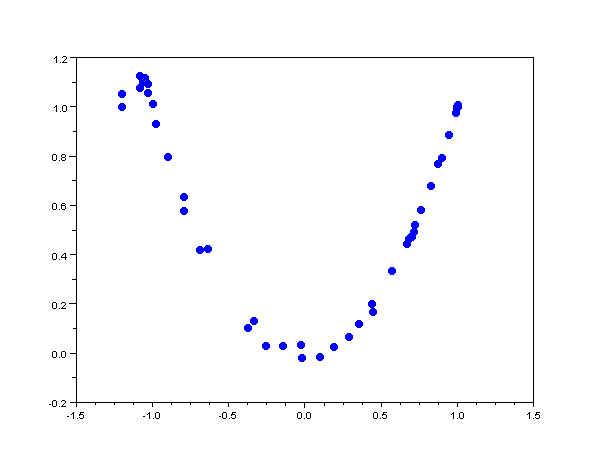
\includegraphics[width=10cm]{fminsearch/testFminsearchPlotScilab.png}
\end{center}
\caption{Plot produced by Scilab's fminsearch, with customized output function.}
\label{fig-fminsearch-scilab-outputfun}
\end{figure}

Except for the size of the dots (which can be configured in 
both softwares), the graphics are exactly the same.

Scilab also prints the following messages in the console.

\lstset{language=scilabscript}
\begin{lstlisting}
// Scilab
3 2.420000e+001 0 -- init
3 2.005000e+001 1 -initial simplex- iter
5 5.161796e+000 2 -expand- iter
7 4.497796e+000 3 -reflect- iter
9 4.497796e+000 4 -contract outside- iter
11 4.381360e+000 5 -contract inside- iter
13 4.245273e+000 6 -contract inside- iter
[...]
149 2.004302e-008 80 -contract inside- iter
151 1.122930e-009 81 -contract inside- iter
153 1.122930e-009 82 -contract outside- iter
155 1.122930e-009 83 -contract inside- iter
157 1.107549e-009 84 -contract outside- iter
159 8.177661e-010 85 -contract inside- iter
159 8.177661e-010 85 -- done
\end{lstlisting}

We see that the output produced by the two software are identical,
expect for the two first lines and the last line.
The lines \#1 and \#2 are different is because Scilab computes the 
function values of all the vertices before calling back the output function.
The last line is different because Scilab considers that once the optimization
is performed, the type of the step is an empty string. Instead, Matlab
displays the type of the last performed step.

\subsection{Predefined plot functions}

\index{optimplotfval}
\index{optimplotx}
\index{optimplotfunccount}

Several pre-defined plot functions are provided with 
the \scifunction{fminsearch} function.
These functions are 
\begin{itemize}
\item \scifunction{optimplotfval},
\item \scifunction{optimplotx},
\item \scifunction{optimplotfunccount}.
\end{itemize}

In the following Matlab script, we use the \scifunction{optimplotfval}
pre-defined function.
\index{optimset}

\lstset{language=matlabscript}
\begin{lstlisting}
% Matlab
options = optimset('PlotFcns',@optimplotfval);
[x fval] = fminsearch(banana , [-1.2, 1] , options)
\end{lstlisting}

The previous script produces the plot which is presented in figure 
\ref{fig-fminsearch-matlab-optimplotfval}.

\begin{figure}
\begin{center}
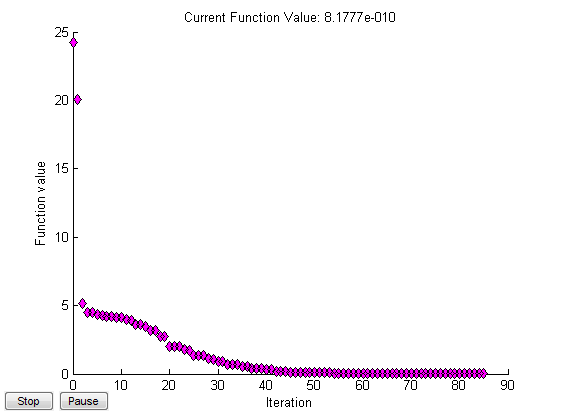
\includegraphics[width=10cm]{fminsearch/testFminsearchOptimplotfvalMatlab.png}
\end{center}
\caption{Plot produced by Matlab's fminsearch, with the \scifunction{optimplotfval} function.}
\label{fig-fminsearch-matlab-optimplotfval}
\end{figure}

The following Scilab script uses the \scifunction{optimplotfval}
pre-defined function.
\index{optimset}

\lstset{language=scilabscript}
\begin{lstlisting}
// Scilab
opt = optimset ( "OutputFcn" , optimplotfval );
[x fval] = fminsearch ( banana , [-1.2 1] , opt );
\end{lstlisting}

The previous script produces the plot which is presented in figure 
\ref{fig-fminsearch-scilab-optimplotfval}.

\begin{figure}
\begin{center}
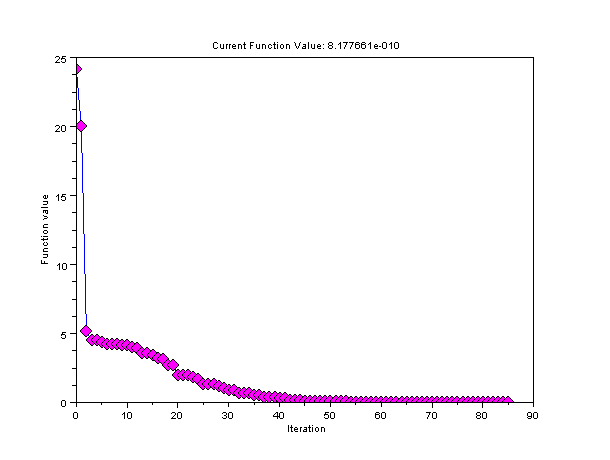
\includegraphics[width=10cm]{fminsearch/testFminsearchOptimplotfvalScilab.png}
\end{center}
\caption{Plot produced by Scilab's fminsearch, with the \scifunction{optimplotfval} function.}
\label{fig-fminsearch-scilab-optimplotfval}
\end{figure}

The comparison between the figures \ref{fig-fminsearch-matlab-optimplotfval} and 
\ref{fig-fminsearch-scilab-optimplotfval} shows that the two features produce
very similar plots. Notice that Scilab's \scifunction{fminsearch} does not 
provide the "Stop" and "Pause" buttons.

The figures \ref{fig-fminsearch-scilab-optimplotx} and \ref{fig-fminsearch-scilab-optimplotfunccount}
present the results of Scilab's \scifunction{optimplotx} and \scifunction{optimplotfunccount}
functions.

\begin{figure}
\begin{center}
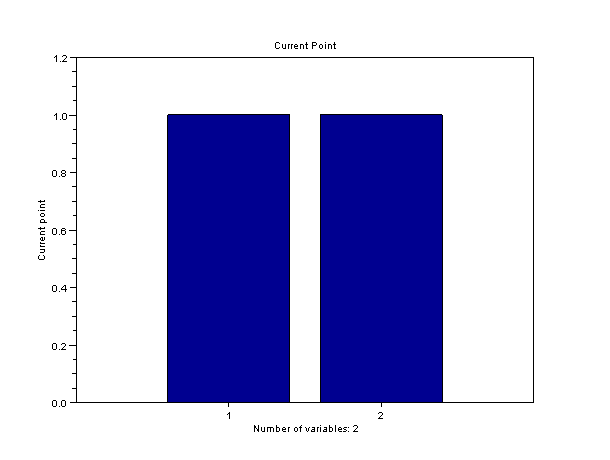
\includegraphics[width=10cm]{fminsearch/testFminsearchOptimplotxScilab.png}
\end{center}
\caption{Plot produced by Scilab's fminsearch, with the \scifunction{optimplotx} function.}
\label{fig-fminsearch-scilab-optimplotx}
\end{figure}

\begin{figure}
\begin{center}
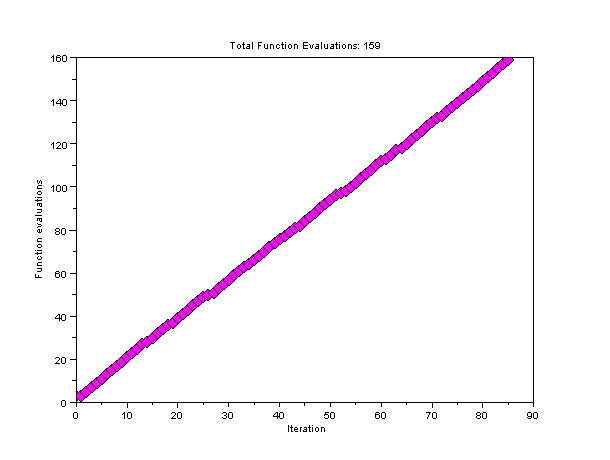
\includegraphics[width=10cm]{fminsearch/testFminsearchOptimplotfunccountScilab.png}
\end{center}
\caption{Plot produced by Scilab's fminsearch, with the \scifunction{optimplotfunccount} function.}
\label{fig-fminsearch-scilab-optimplotfunccount}
\end{figure}

\section{Conclusion}

The current version of Scilab's \scifunction{fminsearch} provides the same algorithm
as Matlab's \scifunction{fminsearch}. The numerical precision is the same.
The \scifunction{optimset} and \scifunction{optimget} functions allows to configure the optimization, 
as well as the output and plotting function.
Pre-defined plotting function allows to get a fast and nice plot of the optimization.




\clearpage

%% Bibliography

\addcontentsline{toc}{chapter}{Bibliography}
\bibliographystyle{plain}
\bibliography{neldermead}

% Index
\addcontentsline{toc}{chapter}{Index}
\printindex

\end{document}

